\section{Introduction and Motivation}

Advances in machine learning are driven by open, easy-to-use libraries that let researchers focus on developing frontier architectures. For example, deep learning research was propelled by Caffe~\citep{DBLP:conf/mm/JiaSDKLGGD14}, TensorFlow~\citep{DBLP:conf/osdi/AbadiBCCDDDGIIK16} and PyTorch~\citep{DBLP:conf/nips/PaszkeGMLBCKLGA19}. Similarly, developments in graph machine learning~\citep{kipfsemi,velivckovic2017graph, DBLP:journals/corr/abs-2012-09699,rampavsek2022recipe} are accelerated by libraries such as PyG~\citep{DBLP:journals/corr/abs-1903-02428, DBLP:journals/corr/abs-2507-16991} and DGL~\citep{wang2019deep}. However, both PyG and DGL are designed for static graphs and cannot capture the temporal dynamics of networks, known as Temporal Graphs~(TGs). Real-world examples include transaction~\citep{DBLP:conf/nips/ShamsiVKGA22}, social~\citep{huang2023temporal}, trade~\citep{poursafaei2022towards}, and communication networks~\citep{DBLP:journals/corr/abs-2011-13085} among others. 

Recently, Temporal Graph Learning (TGL) has emerged to capture both spatial and temporal dependencies in networks~\citep{cornell2025power,cao2020spectral,han2014chronos}. The field has seen growth with high-impact, cross-domain applications, such as LinkedIn's LiGNN system~\citep{borisyuk2024lignn} for user recommendations and mobility modelling that informed COVID-19 policy decisions~\citep{chang2021mobility}. Unlike static graph ML, TGL must treat time as a first-class signal, making timestamps central to modelling and data processing. Despite research progress, software infrastructure has not kept pace.


\textbf{Limitations of existing libraries.} Current TG libraries~\citep{dygfomer,DBLP:conf/cikm/RozemberczkiSHP21} are narrow in scope: many implement only a single algorithm family~\citep{10.1145/3620665.3640414, DBLP:conf/sc/ZhouZSKP23} and most lack extensibility, resulting in a fragmented ecosystem. For instance, TGL~\citep{DBLP:journals/corr/abs-2203-14883}, DistTGL~\citep{DBLP:conf/sc/ZhouZSKP23} and TGLite~\citep{10.1145/3620665.3640414} are optimized for temporal message passing architectures~\citep{tgn,tgat} but do not support emerging transformer-based approaches~\citep{dygfomer,DBLP:journals/corr/abs-2507-11836}. Also, none provide time conversion operations which are critical for analyzing temporal granularity in TGs~\citep{utg}. Finally, existing libraries fall short on usability features needed to foster reproducible research such as profiling tools, test suites, and modular abstractions (see Table~\ref{tab:features}).

\textbf{Motivation for a unified framework.} Unlike NLP, where the transformer serves as a canonical architecture~\citep{vaswani2017attention}, TGL lacks a standard model family. This leads to fragmented and error-prone experimentation: continuous- and discrete-time models require entirely different data pipelines, while core operations such as temporal neighbor sampling and negative edge construction are implemented inconsistently. Without a unified framework, the community faces difficulties in fair benchmarking, rapid prototyping, and combining ideas across approaches.

\textbf{Our solution.} We introduce \name, a modular and efficient framework for TGL research. \name introduces several firsts: native support for node events, a generic hook mechanism that standardizes TG transformations, and unified support for both continuous- and discrete-time graphs, ending the long-standing separation between the two lines of research~\citep{tgn,DBLP:conf/kdd/YouDL22}. Node events naturally capture phenomena like social media posts or other user activity in real-world networks~\citep{DBLP:journals/jmlr/KazemiGJKSFP20}. These abstractions unify diverse TG pipelines, lowering the barrier for practitioners and accelerating innovation. Beyond flexibility, \name delivers efficiency: $7.8\times$ faster than DyGLib on standard TG models and an average speedup of $175\times$ on graph discretization.


% {\vspace{-5em}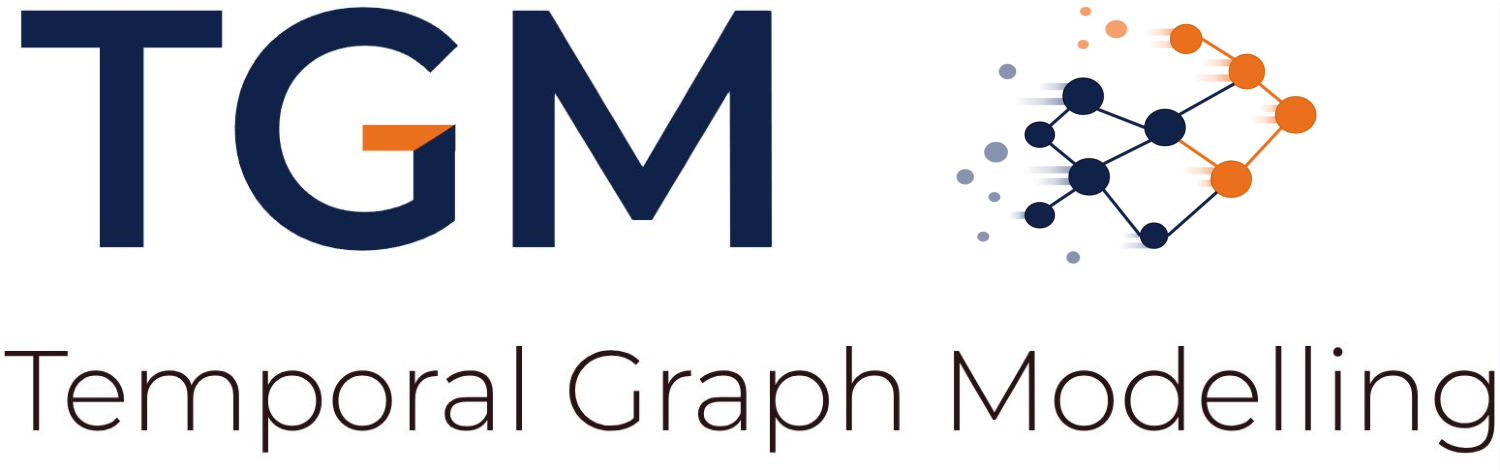
\includegraphics[width=10cm]{iclr_2026/artifacts/logo/logo-high-res.pdf}
% }

\begin{figure}
    \centering
    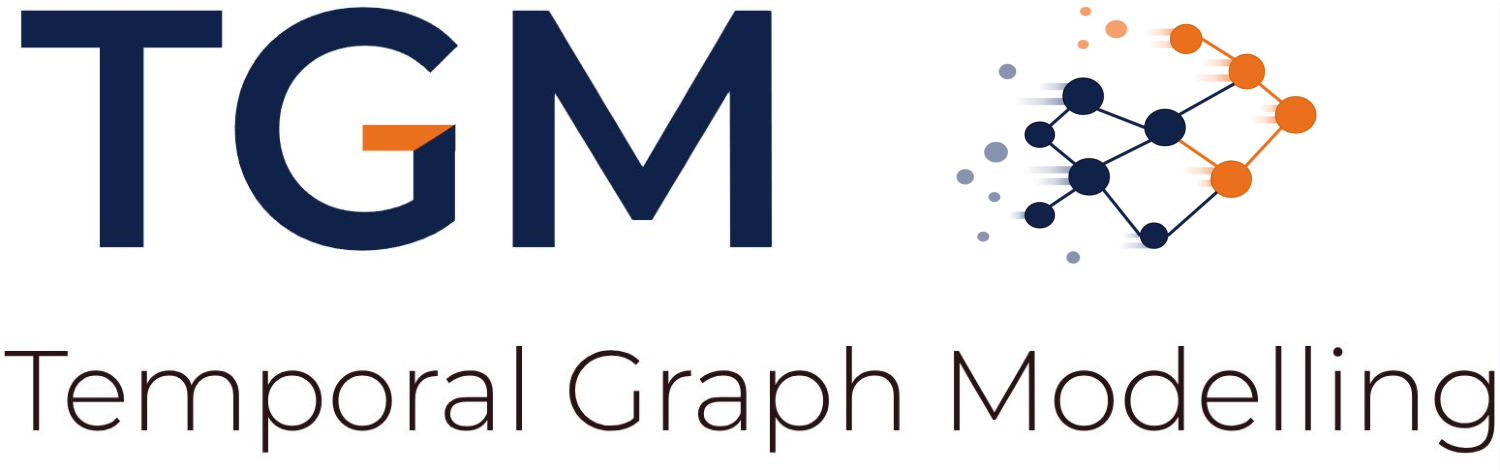
\includegraphics[width=0.7\textwidth]{iclr_2026/artifacts/logo/logo-high-res.pdf}
    \vspace{-1.2em}
\end{figure}

\begin{figure*}[t]
  \centering
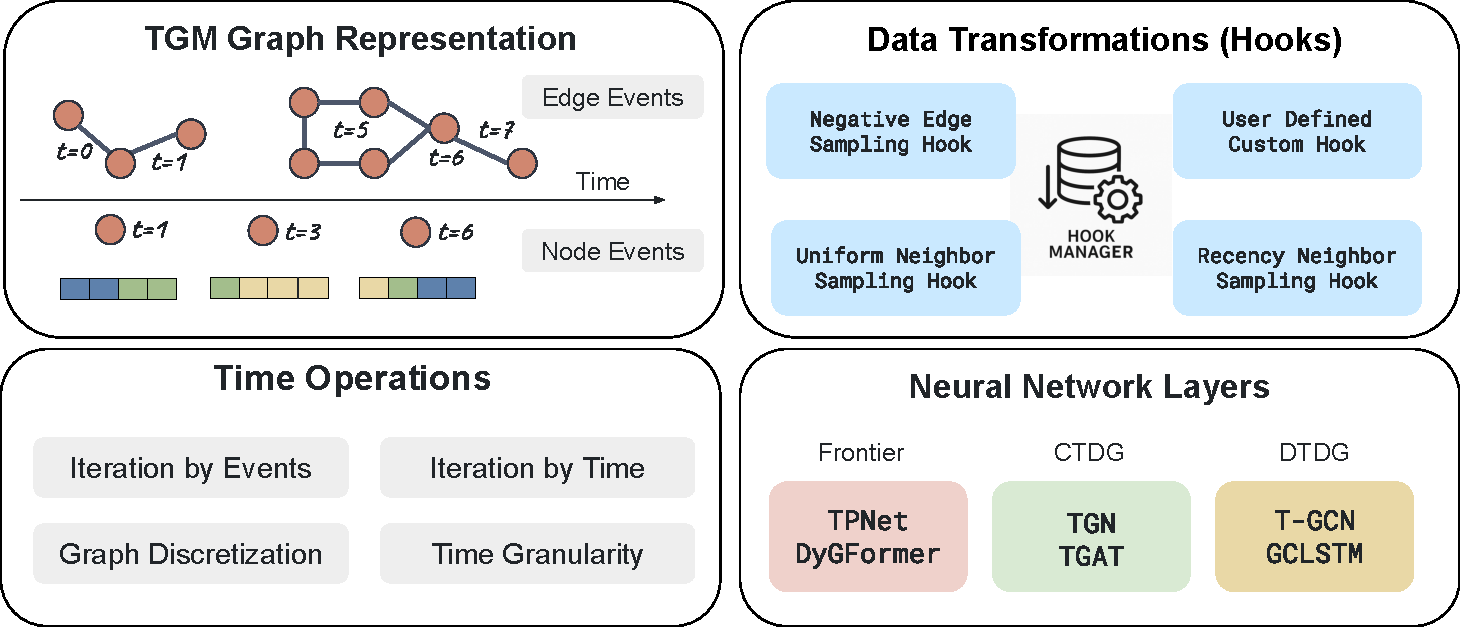
\includegraphics[width=0.9\linewidth]{iclr_2026/artifacts/tgm_features.pdf}
  \caption{Overview of \name features. \name has native support for node events and unified continuous- and discrete-time graph iteration (left). Generic hooks formalize common TG transformations (top-right). \name supports a broad range of temporal graph learning methods (bottom-right).}
  \label{fig:paradigm}
\end{figure*}


In summary, the key properties of \name are:
\begin{itemize}[leftmargin=*, noitemsep, topsep=0.2pt]
    \item \textbf{First unified library for TG.} \name is the first library to support both continuous- and discrete-time graphs, treating them as distinct views of the same underlying data. We implement 8 methods from both CTDG and DTDG literature, including frontier models.

    \item \textbf{Time as a first-class citizen.} Time operations are central to TGs. \name natively incorporates time granularity into its API, with built-in support for graph discretization and snapshot iteration.

    \item \textbf{Efficiency.} Our experiments show that \name achieves an average $7.8\times$ faster end-to-end training than DyGLib, and $175\times$ faster graph discretization compared with existing implementations.

    \item \textbf{Research-oriented.}  Designed for rapid prototyping, \name emphasizes modularity and ease-of-use. Its novel hook mechanism standardizes temporal graph transformations while supporting the broadest range of TG tasks: link, node, and graph-level prediction. 
\end{itemize}

